%%   This file is part of the APS files in the REVTeX 4 distribution.
%%   Version 4.0 of REVTeX, August 2001
%%
%%
%%   Copyright (c) 2001 The American Physical Society.
%%
%%   See the REVTeX 4 README file for restrictions and more information.
%%
%
% This is a template for producing manuscripts for use with REVTEX 4.0
% Copy this file to another name and then work on that file.
% That way, you always have this original template file to use.
%
% Group addresses by affiliation; use superscriptaddress for long
% author lists, or if there are many overlapping affiliations.
% For Phys. Rev. appearance, change preprint to twocolumn.
% Choose pra, prb, prc, prd, pre, prl, prstab, or rmp for journal
%  Add 'draft' option to mark overfull boxes with black boxes
%  Add 'showpacs' option to make PACS codes appear

% Edited by Camilla Harris Jan 2015
% For use by Camilla Harris, Akshat Mahajan
% in creating Lab Reports for 180c at UCLA
% this file and auxiliary files were retrieved from
% http://www-d0.fnal.gov/Run2Physics/WWW/templates/
% on Jan 19 2015

\documentclass[aps,prl,nofootinbib,twocolumn,superscriptaddress,groupedaddress]{revtex4}  % for review and submission
%\documentclass[aps,preprint,superscriptaddress,groupedaddress]{revtex4}  % for double-spaced preprint
% CAMILLA: I removed the PACS functionality
\usepackage{graphicx}  % needed for figures
	%if using postscript files compile with XeLaTex
\usepackage{dcolumn}   % needed for some tables
\usepackage{bm}        % for math
\usepackage{amssymb}   % for math
\usepackage[export]{adjustbox}
\usepackage{array}
\usepackage{multirow, bigdelim}

% avoids incorrect hyphenation, added Nov/08 by SSR
\hyphenation{ALPGEN}
\hyphenation{EVTGEN}
\hyphenation{PYTHIA}

\begin{document}
\title{Observing the Quantum Hall Effect}
\input author_list.tex        % includes institutions and visitors
\date{\today}

\begin{abstract}
Measurements of the transverse and longitudinal resistivity of a GaAs-based heterostructure for small current ($<$ 0.1 $\mu$A) were made at low temperature while exposed to a range of magnetic fields (upto 9 T). The transverse resistivity exhibited integer quantisation (the integer quantum Hall effect) whereas the longitudinal resistivity exhibited the so-called Shubnikov-de Haas oscillations. We derive the fine structure constant ($7.231 \times 10^{-3}$) and the electron density of our heterostructure from this information.
\end{abstract}

\maketitle

\section{Background Information}
In classical physics, a magnetic field applied perpendicular to a current-carrying sample causes the sample to develop a voltage perpendicular to the current and the field. This is the so-called \textsl{Hall voltage}, typically arising from the interaction of the magnetic field with the electrons that constitute the current passing through the sample. Charges, on encountering a magnetic field, develop a curved trajectory - they begin to accumulate along the edges of the sample, inducing an electric field along the edges that are perpendicular to the sample's current. A schematic overview of this effect is presented in Fig. 1. The classical Hall voltage $V_{H}$ is given by\cite{nobel} \begin{equation}
V_{H} = \frac{I_{ch}B}{nte}
\end{equation}
where $I_{ch}$ is the sample current, $B$ is the applied field, $t$ refers to the sample thickness, $n$ is the electron density of the sample, and $e$ is the absolute value of the electron charge. 

\begin{figure}[b]
\centering
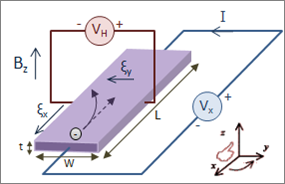
\includegraphics[scale = 0.9]{Hall.PNG}
\caption{Classical Hall effect. The magnetic field $B_{z}$ in the $z$-direction generates an electric field component $E_{y}$ in the y-direction from the current $I$. The Hall voltage arises by multiplying $E_{y}$ with the sample width.}
\end{figure}

Typically, the classical picture holds extremely well at room temperatures. However, at low temperatures ($<$ 10 K), it becomes clear that the Hall voltage  is \textit{quantized}\cite{lab}:
\begin{equation}
V_{H} = \frac{I_{ch}h}{\nu e^{2}}
\end{equation}
where $h$ is Planck's constant and $\nu$ is an integer ($\nu = 1, 2, 3 \ldots$). This is in direct contrast with the classical picture, which varies directly with the field strength. The quantum Hall effect, as it is known, occurs semiclassically because the electron density $n$ in Eq. 1. becomes quantised when exposed to a magnetic field \cite{lab} - thus, the classical $V_{H}$ transitions smoothly to a quantum $V_{H}$.

In this paper, we reproduce the quantum Hall effect experimentally. A 3 mm x 1 mm GaAs-based heterostructure was subjected to 2 K, 4 K and 7 K temperatures using a helium-3 cooled refrigerating system, and its transverse and longitudinal resistances measured as a function of magnetic field strength as 100 nA were passed through the sample. The magnetic field was varied continuously between 0 - 9 T. A simplified overview of the measurement apparatus is provided below; in practice, the measurement apparatus was a commercial instrument called the Physical Property Measurement System (PPMS), sold by Quantum Design\cite{qd}. The system typically performs a 5-wire Hall effect measurement (not shown in Fig. 2), and is sensitive to fluctuations on the order of 10 nV. The resistances were measured every 0.1 T (in other words, 90 steps between 0 to 9 T). 

\begin{figure}[b]
\centering
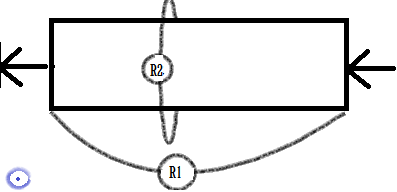
\includegraphics[scale=0.8]{InstrumentOverview.png} 
\caption{Simplified drawing of measurement apparatus. The arrows indicate the direction of current, $R2$ refers to the transverse resistance, and $R1$ refers to the longitudinal resistiance. In practice, $R2$ and $R1$ were a collection of voltmeters and ammeters that enabled determination of resistance. The blue circle represents the direction of the magnetic field.}
\end{figure}

The GaAs-based heterostructure used consisted of a layer of AlGaAs n-doped with Si atoms, separated from the ionized donor by an undoped AlGaAs spacer of thickness of 5 nm, covered still further by an NiCr conducting gate situated 300 nm from the electron layer and insulated from the undoped AlGaAs layer. A thin layer of GaAs covered the sample on both sides to prevent electron diffusion into surrounding layers. This heterostructure is frequently used and cited in the literature for the Hall effect as its electronic behaviour can easily be approximated as a two-dimensional electron gas\cite{lab,nobel}, allowing for clean and accurate measurements of the Hall effect. Fig. 3 presents a graphical overview of the heterostructure. 

\begin{figure}[t]
\centering
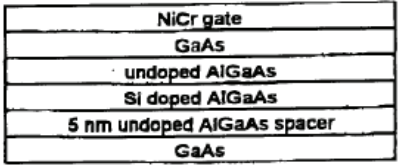
\includegraphics[scale=0.8]{Heterostructure.png} 
\caption{The GaAs-based heterostructure used in our experiment\cite{lab}.}
\end{figure}

\section{Results}

Fig. 4 demonstrates our results. All measurements were initially made in Ohms ($\Omega$) - for the purposes of clarity and independence of geometry, they were converted to units of resistivity ($\Omega$ m). Conversion was obtained as 
\begin{equation}
\rho_{l} = \frac{AR_{l}}{\ell} = \frac{3\mathrm{mm} \times 1 \mathrm{mm} \times R_{l}}{3 \mathrm{mm}} = 10^{-3} \mathrm{m} \times R_{l} 
\end{equation}
where the subscript $l$ refers to corresponding longitudinal quantities, and
\begin{equation}
\rho_{t} = \frac{AR_{t}}{\ell} = \frac{3\mathrm{mm} \times 1 \mathrm{mm} \times R_{t}}{1 \mathrm{mm}} = 3 \times 10^{-3} \mathrm{m} \times R_{t}
\end{equation}
where the subscript $t$ refers to corresponding transverse quantities. We have used the definition of resistivity to obtain these conversions. $A$ and $\ell$ refer to the cross-sectional area and the directed length (transverse or longitudinal) respectively. The Hall voltage graphs are derived from transverse resistance, using Ohm's law:
\begin{equation}
V_{H} = I_{ch}\times R_{t} = 100 \mathrm{nA}\times R_{t} = 100 \times 10^{-6} \times R_{t} \mathrm{mV}
\end{equation}

\onecolumngrid

\begin{figure}[b]
\centering
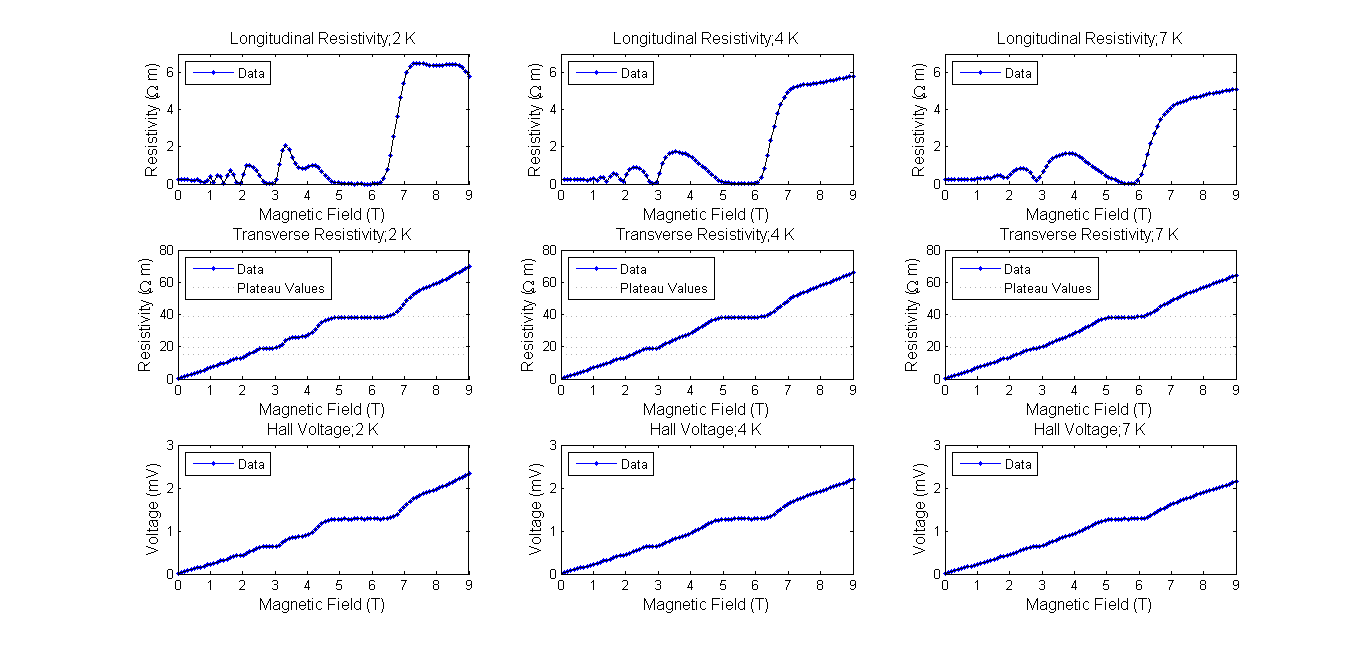
\includegraphics[width = \textwidth]{../Analysis/ChannelsVField.png}
\caption{A 3x3 column grid displaying the results of measuring the transverse and longitudinal resistances. The first row demonstrates the famous Shubnikov-de Haas oscillations; the second row demonstrates the quantized  transverse resistivity; the third row demonstrates the quantised nature of the Hall voltage. Troughs in the Shubnikov-de Haas oscillations correspond to plateaus in the resistance and the Hall voltage. Horizontal lines are plateau values predicted from Eq. 6.}
\end{figure}

\twocolumngrid

We note that the longitudinal resistivity oscillates with growing amplitude as the magnetic field increases - these are referred to as the Shubnikov-de Haas oscillations, and can be theoretically explained by the same semi-classical treatment that leads to the quantised Hall effect\cite{lab}. They are relatively consistent over different temperatures. Further, comparison with Eq. 2 and the actual data tells us the transverse resistivity $\rho_{t}$ can be described by \begin{equation}
\rho_{t} = \frac{AV}{\ell I_{ch}} = \frac{Ah}{\ell\nu e^{2}} = \frac{77.438}{\nu} \,\,\Omega \mathrm{m}
\end{equation} 
\begin{table}[t]
\caption{Plateau values derived from Eq. 6 shown on graph for 2 K, alongside corresponding magnetic field ranges. All units are $\Omega$ m or Tesla respectively.}
\begin{ruledtabular}
\begin{tabular}{cccc}
$\nu$ & $\rho_{t}$& Plateau Start (T) & Plateau End(T)\\
2 & 38.741& 5.056 & 6.472 \\
3 & 25.827& 3.640 & 3.742 \\
4 & 19.370 & 2.629 & 3.034 \\
5 & 15.496 & 2.225 & 2.225 \\
\end{tabular}
\end{ruledtabular}
\end{table}

\begin{table}[t]
\caption{Plateau values derived from Eq. 6 shown on graph for 4 K, alongside corresponding magnetic field ranges. All units are $\Omega$ m or Tesla respectively.}
\begin{ruledtabular}
\begin{tabular}{cccc}
$\nu$ & $\rho_{t}$& Plateau Start (T) & Plateau End(T)\\
2 & 38.741& 5.157 & 6.270 \\
3 & 25.827& 3.640 & 3.640 \\
4 & 19.370 & 2.730 & 3.034 \\
5 & 15.496 & 2.225 & 2.225 \\
\end{tabular}
\end{ruledtabular}
\end{table}

\begin{table}[b]
\caption{Plateau values derived from Eq. 6 shown on graph for 7 K, alongside corresponding magnetic field ranges. All units are $\Omega$ m or Tesla respectively.}
\begin{ruledtabular}
\begin{tabular}{cccc}
$\nu$ & $\rho_{t}$& Plateau Start (T) & Plateau End(T)\\
2 & 38.741& 5.461 & 6.067 \\
3 & 25.827& 3.742 & 3.742 \\
4 & 19.370 & 2.831 & 2.933 \\
5 & 15.496 & 2.225 & 2.225 \\
\end{tabular}
\end{ruledtabular}
\end{table}
\vspace{-4\baselineskip}
\section{Analysis}
In order to determine the start and end values for our plateaus, the plateau values were first theoretically derived using Eq. 6, and then compared to the data. Points closest in value (i.e. within 0.5 $\Omega$ m of the theoretical value) were chosen and the slope between each neighbouring point compared. Those with forward slope (i.e. slope with the point after them) much smaller than backward slope (i.e. slope calculated with the point before them) were taken to be the start of the plateau; those with backward slope smaller than forward slope were similarly taken to be the end of the plateau. Since this situation can occur for even small fluctuations of data within the plateaus and does not guarantee uniqueness, those points with the most pronounced difference between forward and backward slopes were ultimately chosen to be the start and the end of the plateau. Tables I, II and III present our results for the three temperatures we studied. At times, only one point could be found within 0.5 $\Omega$ m of the theoretical plateau value, and was correspondingly marked both the start and end points of that plateau. Where the difference between start and end points is zero, however, it is safe to say that that plateau was not sufficiently developed.

This clean treatment allows us to smoothly estimate the density of electrons $n$. From comparison with Eq. 1 and 2, we can say that 
\begin{equation}
n \propto \frac{\nu e B}{h} = 2.417 \times 10^{14}\times \nu \times B \; \textrm{m}^{-2}
\end{equation}
More detailed derivations for this result\cite{nobel} have discovered that the proportionality constant for this relationship is in fact 1 (in other words, sample thickness $t$ is not a parameter) for T = 0. Assuming that this equation can validly describe deviations from T = 0, we take the average of our start and end points to arrive at $B$ for the corresponding $\nu$. Table IV contains our results. We obtain an estimate of 
$$ n = (272 \times 10^{15} \pm 5.44) \times 10^{13} \; \mathrm{m}^{-2}$$
from averaging and computing the standard deviation of the values in Table IV. This is fairly reasonable - the large standard deviation is much smaller than the mean value, so that in reality the values of $n$ are very closely clustered together. However, the accuracy of this result depends very much on how accurate Eq. 7 continues to be at close to zero temperature.
\begin{table}[b]
\caption{Electron density $n$ derived from Eq. 7 for different temperatures and $\nu$.}
\begin{ruledtabular}
\begin{tabular}{ccc}
$\nu$ & Temperature & $n$ (m$^{-2}$)\\
\hline
\hline
2 & 2 K& $2.78 \times 10^{15}$ \\
2 & 4 K& $2.76 \times 10^{15}$ \\
2 & 7 K& $2.78 \times 10^{15}$ \\
3 & 2 K& $2.67 \times 10^{15}$ \\
3 & 4 K& $2.63 \times 10^{15}$ \\
3 & 7 K& $2.71 \times 10^{15}$ \\
4 & 2 K& $2.73 \times 10^{15}$ \\
4 & 4 K& $2.78 \times 10^{15}$ \\
4 & 7 K& $2.78 \times 10^{15}$ \\
5 & 2 K& $2.68 \times 10^{15}$ \\
5 & 4 K& $2.68 \times 10^{15}$ \\
5 & 7 K& $2.68 \times 10^{15}$ \\
\end{tabular}
\end{ruledtabular}
\end{table}

In turn, we can proceed to derive the fine structure constant $\alpha$ from our values of the resistivity. It can be shown that\cite{nobel} 
\begin{equation}
\alpha = \frac{\mu_{0} c}{2 R_{H} \nu} = \frac{\mu_{0} c A}{2\rho_{t}\ell\nu} = 0.56 \times \frac{1}{\rho_{t}\nu} 
\end{equation}

Because our plateau values were determined from Eq. 6 in the first place, we find that $\frac{1}{\rho_{t}\nu} =  \frac{1}{77.438}$, so that our value of $\alpha$ is just $7.231 \times 10^{-3}$. This differs from the correct value of $7.297 \times 10^{-3}$, although not substantially. It is likely that the errors in estimating the area and length of our sample have propagated to provide this value. In the absence of more accurate measurements of area and length, however, we report this value as our official figure.

\begin{figure}[t]
\centering
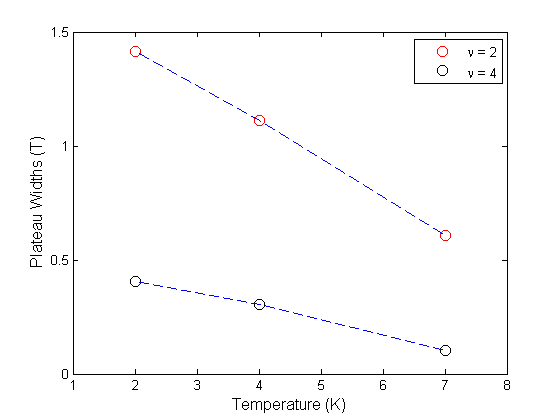
\includegraphics[scale = 0.6]{../Analysis/plateauwidths.png}
\caption{A plot of plateau width versus temperature for different plateaus. Only $\nu = 2,4$ were consistently non-zero throughout and hence are displayed here.} 
\end{figure}

The effect of temperature on the Hall effect is as follows: at low temperatures, the plateau widths are larger than at high temperatures. The full reason for this arises from a proper quantum-mechanical treatment. Further, our expression (Eq. 7)  for electron density $n$ is theoretically valid at T = 0; from Fermi-Dirac statistics, we know that the electron density $n$ is really obtained by integrating the Fermi-Dirac distribution $f(T,E)$ multiplied by the density of states $\mathrm{DOS}(E)$ i.e. \begin{equation}
n(E) = \int_{0}^{\infty}\mathrm{DOS}(E)f(T,E) dE
\end{equation}
where $$f(T,E) = \frac{1}{1 + e^{\frac{E - E_{F}}{kT}}}$$. Here, $k$ is the Boltzmann constant, $E$ the energy, $T$ the temperature, and $E_{F}$ the Fermi energy. For small $T$ and for a 2D density of states (appropriate since our system is essentially a two-dimensional electron gas), we can argue that $$n \approx \frac{\nu e B}{h}\int_{0}^{\infty}\exp^{\frac{E_{F} - E}{kT}} dE$$
from which we can obtain from a semi-classical treatment 
\begin{equation}
\rho_{t} \approx \frac{Ah}{\ell\nu e^{2}}\int_{0}^{\infty}\exp^{\frac{E - E_{F}}{kT}} dE
\end{equation}

While this expression by itself is not sufficient to characterise the plateau widths, it does suggest that the quantum hall effect is affected by temperature. Toyoda \textit{et al.}\cite{toyoda} and Isihara\cite{isihara} have advanced theoretical explanations that argue that the decrease in plateau width with temperature is roughly linear for small $T$. Empirically, Tables I, II and III demonstrate that the plateau width decreases with temperature. This is shown more clearly in Fig. 5.

Now we discuss the effects of electron spin on the quantum Hall effect. The energy levels of a bound electron within an external magnetic field split into two levels, one for spin up and the other for spin down electrons, which differ from the original energy level by $\pm\frac{ge\hbar B}{2m_{e}}$ in energy, where $B$ is the magnetic field and $g$ the Lande factor. This is the \textit{Zeeman} effect, and it affects Landau levels (the energy states corresponding to our system). As a consequence, for every $N$ Landau levels initially in close-to-zero external field, there now exist 2$N$ Landau levels. The spin-split levels can overlap between different Landau levels, and thus be treated as localised states in their own right. The most important consequence of this is that it leads to the formation of visible additional plateaus (these are odd-integer plateaus where $\nu = 1, 3, 5 \ldots$) at low temperatures\cite{murzin}.  One can see this in the data for 2 K, where $\nu = 3$ is clearly resolved as a true plateau. Strong disorder effects, however, tend to smear this out for higher temperatures\cite{murzin}.

Finally, we move on to discuss how to obtain the electron density $n$ from the longitudinal resistivity data. For every magnetic field $B_{p}$ at the crest of oscillation $p$, the electron density is given by $$n = \frac{qe}{h}\left[\frac{1}{B_{p + 1}} - \frac{1}{B_{p}}\right]^{-1}$$
where $q$ is 1 for unsplit and 2 for spin-split levels respectively. The values $B_{p}$ were collected using MATLAB's peak-finding algorithm. We chose to examine only unsplit levels for convenience, and restricted our attention to values taken from 7 K and 4 K values. We obtain $$n = (147.40 \pm 23.33) \times 10^{13} \; \mathrm{m}^{-2}$$ 

\begin{table}[t]
\caption{Longitudinal resistivity data. All magnetic fields in Tesla.}
\begin{ruledtabular}
\begin{tabular}{ccccc}
$p$ & Temperature & $B_{p}$ & $B_{p-1}$ & $n (\mathrm{m}^{-2}) $\\
\hline
\hline
2 & 7 K & 2.427 & 1.618 & $1.17 \times 10^{15}$\\
3 & 7 K & 3.843 & 2.427 & $1.59 \times 10^{15}$\\
3 & 4 K & 1.618 & 1.315 & $1.69 \times 10^{15}$\\
4 & 4 K & 2.326 & 1.618 & $1.28 \times 10^{15}$\\
5 & 4 K & 3.539 & 2.326 & $1.64 \times 10^{15}$\\
\end{tabular}
\end{ruledtabular}
\end{table}
\vspace{-2\baselineskip}
\section{Conclusion}
In this paper, we have arrived at two seemingly contradictory values of the electron density, which is not easily explained. A proper assessment of the errors involved in the methods employed is needed. However, our measurement of $\alpha$ is in agreement with the accepted value of $7.297 \times 10^{-3}$.
\begin{thebibliography}{2}

\bibitem{lab}
    \textit{Quantum Hall Effect}, Stuart Brown, Physics 180C lab manual of UCLA.

\bibitem{nobel}
    \textit{The Quantized Hall Effect}, Klaus von Klitzing, Nobel lecture, December 9, 1985, Max-Planck-Institut für Festkörperforschung, D-7000 Stuttgart 80. http://www.nobelprize.org/nobel\_ prizes/physics/laureates/1985/klitzing-lecture.html

\bibitem{toyoda}
    \textit{The Plateau Widths of the Quant1zed Hall Conductance}, T. Toyoda, V. Gudmundsson \textit{et al.}.Volume 102A, number 3 PHYSICS LETTERS 7 May 1984.
    
\bibitem{isihara}
    \textit{Quantized plateaus of the Hall conductance of 2D electron systems}, A. Isihara. \textsl{Surface Science}, Volume 170, Issues 1–2, 3 April 1986, Pages 267–270.
    
\bibitem{murzin}
    \textit{Spin splitting in the quantum Hall effect of disordered GaAs layers with strong overlap
of the spin subbands}. S. S. Murzin, M. Weiss, \textit{et al.} PHYSICAL REVIEW B 71, 155328, 2005. DOI: 10.1103/PhysRevB.71.155328 

\bibitem{qd}
    Physical Property Measurement System official specifications: http://www.qdusa.com/products/ppms.html
    
\bibitem{picture}
    Picture source: http://en.wikipedia.org/wiki/File:Hall\_ Effect\_ Measurement\_ Setup\_ for\_ Electrons.png
\end{thebibliography}

\end{document}